\section{SIMULATION}
We use the rolling gait as the basic gait for simulations. To verify the adaptability of snake-liked robots under our proposed adaptive control, we conduct simulations on poles with different diameters under the robot simulation platform V-REP.

The simulation process can be divided into two categories: training and motion simulation. And we divide simulations into two parts: the adaptable motion along poles having changing diameter and the adaptable motion along straight poles with different diameters.

\subsection{Training process}

In the data acquisition process, we let the robot climb along the 25\,cm and 35\,cm poles under different parameters and collect 25 thousand volumes of training data in total. The interval of amplitude $A$, phase $\varepsilon$ and angular rate $\omega$ are $[40, \, 80]$, $[0, \, 5]$ and $[1.5, \, 3]$ respectively. What's more, the step of $A$ is 5, the step of $\varepsilon$ is 1 and the step of $\omega$ is 0.5. We make the robot climb poles with different combination of parameters and then collect the data. In the preprocessing process, we cluster the training data. We set the number of clusters as 25 by Eq.\ref{clu_var} and \figref{fig:clusize}. The number of data for most of classes is $1000 \pm 500 $ (\figref{fig:clustersize}).

\begin{figure}[!h]
	\centering
	\includegraphics[width=1.0\linewidth,height=125pt]{fig/experiment/170912/clusize}
	\caption{The variance in cluster size of $N_{k}$}
	\figlabel{fig:clusize}
\end{figure}

\begin{figure}[t]
	\centering
	\includegraphics[width=0.8\linewidth]{fig/experiment/170912/cluster}
	\caption{The result of clustering}
	\figlabel{fig:clustersize}
\end{figure}

\subsection{the autonomous motions along a variable diameter pole}

\begin{figure}[!h]
	\centering
	\subfigure[t=24s]{
		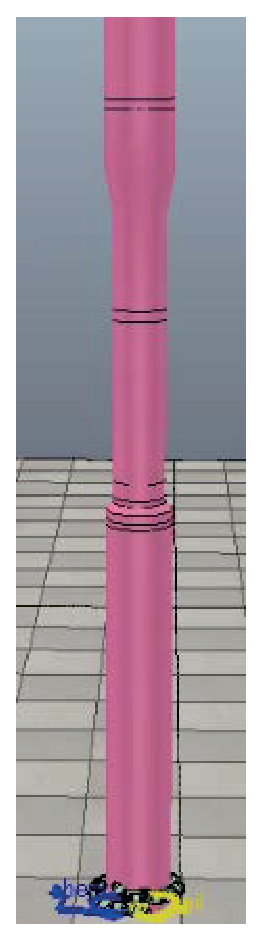
\includegraphics[height=2in,width=.12\textwidth]{fig/experiment/BSB/34s}
	}
	\subfigure[t=35s]{
		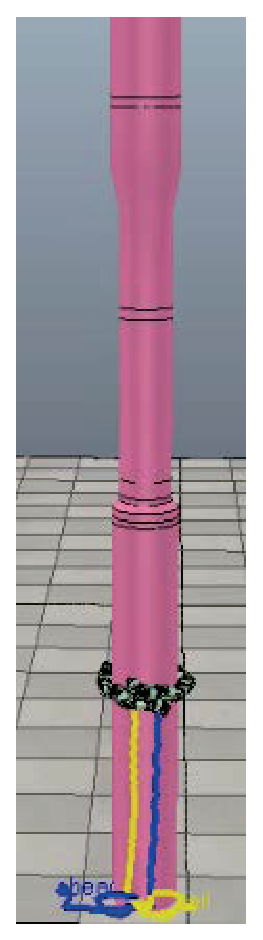
\includegraphics[height=2in,width=.12\textwidth]{fig/experiment/BSB/49s}
	}
	\subfigure[t=47s]{
		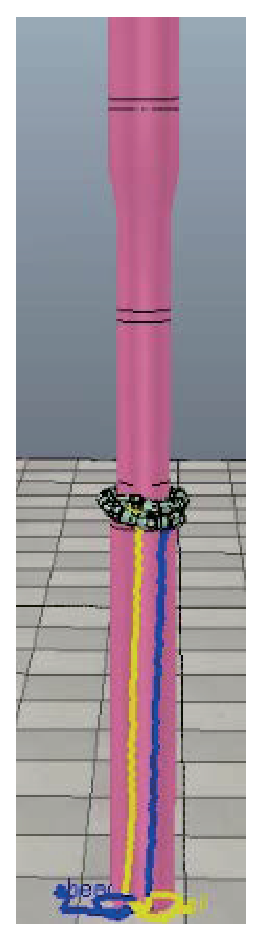
\includegraphics[height=2in,width=.12\textwidth]{fig/experiment/BSB/1m05s}
	}
	\subfigure[t=56s]{
		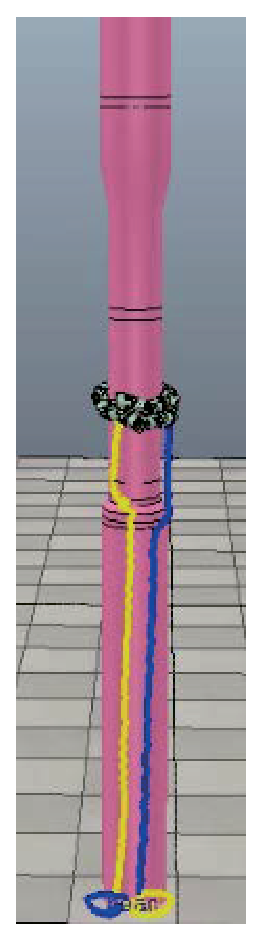
\includegraphics[height=2in,width=.12\textwidth]{fig/experiment/BSB/1m17s}
	}
	\subfigure[t=63s]{
		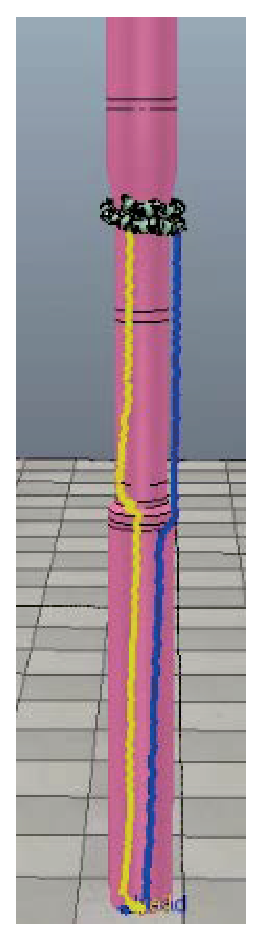
\includegraphics[height=2in,width=.12\textwidth]{fig/experiment/BSB/1m27s}
	}
	\subfigure[t=69s]{
		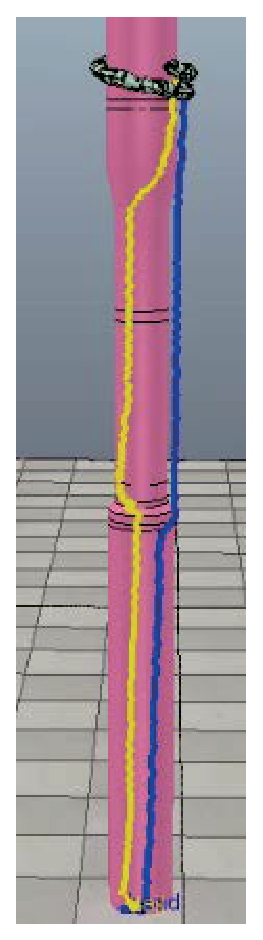
\includegraphics[height=2in,width=.12\textwidth]{fig/experiment/BSB/1m35s}
	}
	
	\subfigure[Amplitude versus Time]{
		\includegraphics[width=114pt,height=95pt]{fig/experiment/BSB/a}
		\figlabel{fig:bsa}
	}
	\subfigure[Phase versus Time]{
		\includegraphics[width=114pt,height=95pt]{fig/experiment/BSB/p}
		\figlabel{fig:bsp}
	}
	
	\subfigure[Angular rate versus Time]{
		\includegraphics[width=114pt,height=95pt]{fig/experiment/BSB/w}
		\figlabel{fig:bsw}
	}
	\subfigure[velocity versus Time]{
		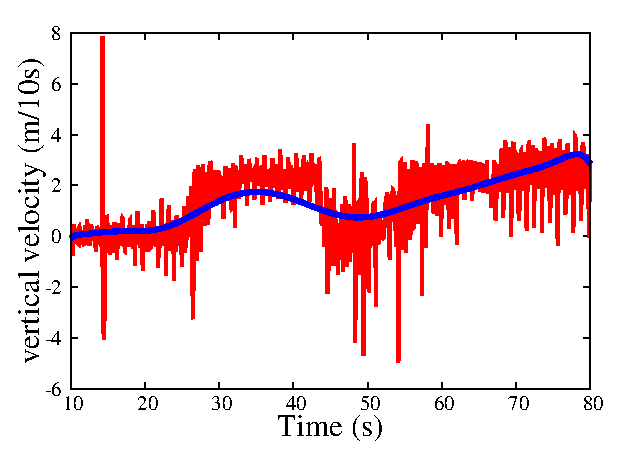
\includegraphics[width=114pt,height=95pt]{fig/experiment/BSB/v}
		\figlabel{fig:bsv}
	}
	\caption{Figure (a) to (f) is the climbing process of the snake-liked robot. Figure (g) to (j) is the parameters curve and velocity curve in climbing.}
	\figlabel{fig:BSB}
\end{figure}
We build a complex pole for simulation in this part. The pole is divided into three sections. The lowest part and the highest part are poles with 35\,cm diameter and the middle part is a pole with 25\,cm diameter. We record the parametes and the velocity during the climbing in 80 seconds.

Results are shown as \figref{fig:BSB}. From 0\,s to 24\,s, the robot changes its shape to  adapt to the unknown pipe. So in this phase, its velocity is close to zero. From 24\,s to 45\,s, the robot climbs along the part with 35\,cm diameter. In this phase, $A$, $\varepsilon$ and $\omega$ are all changing and $A$ and $\varepsilon$ are stable finally. When about 45\,s, the robot reaches the interface where the diameter changes. As the diameter changes obviously, the robot can not grasp the middle part immediately, which causes the velocity of the robot fluctuate around zero. The robot autonomously adjusts its parameters by our strategy to continue its climbing motion. From the \figref{fig:bsa}, \figref{fig:bsp} and \figref{fig:bsw}, it can be found that the parameters are increasing in this phase, which makes the robot continue moving up. Similarly, when about 63\,s, the robot meets the second interface between the middle part and the highest part. The robot maintains its motion by autonomously changing the parameters. And when the robot arrives at the highest part, all the parameters are stable at last. As a whole, the velocity changes toward bigger velocity during the motion.

Eventually all control parameters as well as velocity are stable. It shows that under this control strategy, the robot can adjust its parameters autonomously to adapt to the environment.
%\subsubsection{Simulation about climbing the pipe with 35cm lower diameter and 25cm upper diameter}

%The results are shown in \figref{fig:ccurve1}. From 0s to 15s, the robot change its shape to  adapt to the unknown pipe. So in this phase, its velocity is close to zero. From 15s to 40s, the robot climb along the pipe with 35cm diameter. In this phase, amplitude $A$, phase $\varepsilon$ and angular rate $\omega$ are all increasing and all of the them will be stable finally. About 50s, the robot reach the interface where the diameter changes. As the pipe changes obvious, the robot can not grasp the 25cm pipe immediately, which causes the velocity of the robot fluctuate around zero. The robot keeps learning and autonomously adjust its parameters to continue its climbing motion. From the \figref{fig:bsa} and \figref{fig:bsp}, it can be found that the amplitude and phase are increasing in this phase, which make the robot continue moving up.




%\begin{figure}[!h]
%	\centering
%	\subfigure[t= 0.0s]{
%		\includegraphics[height=2in,width=.12\textwidth]{fig/experiment/170912/sb0}
%	}
%	\subfigure[t=29.2s]{
%		\includegraphics[height=2in,width=.12\textwidth]{fig/experiment/170912/sb1}
%	}
%	\subfigure[t=40.5s]{
%		\includegraphics[height=2in,width=.12\textwidth]{fig/experiment/170912/sb2}
%	}	
%	\subfigure[t=55.0s]{
%		\includegraphics[height=2in,width=.12\textwidth]{fig/experiment/170912/sb3}
%	}
%	\subfigure[t=58.9s]{
%		\includegraphics[height=2in,width=.12\textwidth]{fig/experiment/170912/sb4}
%	}
%	\subfigure[t=66.0s]{
%		\includegraphics[height=2in,width=.12\textwidth]{fig/experiment/170912/sb5}
%	}
%	\subfigure[Amplifier versus Time]{
%		\includegraphics[width=.2\textwidth]{fig/experiment/170912/sbamplifier1}
%		\figlabel{fig:sba}
%	}
%	\subfigure[Phase versus Time]{
%		\includegraphics[width=.2\textwidth]{fig/experiment/170912/sbphase}
%		\figlabel{fig:sbp}
%	}
%	
%	\subfigure[Angular rate versus Time]{
%		\includegraphics[width=.2\textwidth]{fig/experiment/170912/sbangrate}
%		\figlabel{fig:sbw}
%	}
%	\subfigure[velocity versus Time]{
%		\includegraphics[width=.2\textwidth]{fig/experiment/170912/sbv}
%		\figlabel{fig:sbv}
%	}
%	\caption{The movement and the curves of parameters in the motion when the robot climb the pipe with 25cm lower diameter and 35cm upper diameter}
%	\figlabel{fig:ccurve2}
%\end{figure}

%\subsubsection{Simulation about the pipe with 35cm lower diameter and 25cm upper diameter}
%It is similar with the previous simulation, but the movement is different in the interface where the diameter changes. The results are shown in \figref{fig:ccurve2}. About 52s, the robot encounters the interface where the diameter changes. At this time the robot autonomously reduce amplitude slightly (\figref{fig:sba}) and then significantly increase  phase (\figref{fig:sbp}). In this way, the control strategy make the robot move itself from the 25cm part up to the 35cm part. 

The simulations show that our strategy is effective to adapt the robot to climb along the variable diameter pole.

\subsection{Contrast experiments on other straight poles}

As the unknown environment in the real world is complex and volatile, there may be differences between training environment and actual environment. Our training environments are vertical poles with 25\,cm or 35\,cm diameter. To ensure that this control strategy can be applied in real world situation, we conduct several  independent simulations on straight poles whose diameters are 20\,cm, 25\,cm, 30\,cm, 35\,cm or 40\,cm. The result of these simulations are shown in \figref{fig:scurve}. Next is the detailed analysis.

\begin{figure}[!h]
	\centering
%	\subfigure[d=20cm]{
%		\includegraphics[height=2in,width=.12\textwidth]{fig/experiment/170912/D20}
%		\figlabel{fig:D20}
%	}
%	\subfigure[d=25cm]{
%		\includegraphics[height=2in,width=.12\textwidth]{fig/experiment/170912/D25}
%		\figlabel{fig:D25}	
%	}
	
%	\subfigure[d=30cm]{
%		\includegraphics[height=2in,width=.12\textwidth]{fig/experiment/170912/D30}
%		\figlabel{fig:D30}
%	}
%	\subfigure[d=35cm]{
%		\includegraphics[height=2in,width=.12\textwidth]{fig/experiment/170912/D35}
%		\figlabel{fig:D35}
%	}
%	\subfigure[d=40cm]{
%		\includegraphics[height=2in,width=.12\textwidth]{fig/experiment/170912/D40}
%		\figlabel{fig:D40}
%	}	
	\subfigure[Amplitude versus Time]{
		\includegraphics[width=114pt,height=95pt]{fig/experiment/170912/samplifier}
		\figlabel{fig:samplifier}
	}
	\subfigure[Phase versus Time]{
		\includegraphics[width=114pt,height=95pt]{fig/experiment/170912/sphase}
		\figlabel{fig:sphase}
	}
	\subfigure[Angular rate versus Time]{
		\includegraphics[width=114pt,height=95pt]{fig/experiment/170912/sarate}
		\figlabel{fig:sarate}
	}
	\subfigure[velocity versus Time]{
		\includegraphics[width=114pt,height=95pt]{fig/experiment/170912/svel}
		\figlabel{fig:svelocity}
	}
	\caption{Curves about the robot climbing the poles with different diameters}
	\figlabel{fig:scurve}
\end{figure}

By observing the parameter curve we can find that the smaller diameter of the pole is, more time is required to adjust the parameters when the diameter gets smaller. All parameters finally reach a stable value and satisfy the requirements of movement. For the 40\,cm diameter pole, the robot is not long enough to form a single ring to wrap the pole. In this case the influence made by phase $\varepsilon$ is very weak (\figref{fig:sphase}). For the 20\,cm diameter pole, it is difficult for the robot to climb along the pole if we only increase the amplitude $A$, because a too large amplitude will cause the snake-liked robot curling up to a high degree, which is not conducive to climb. Therefore, to let the robot climb the pole with small diameters, we need to constantly adjust the phase $\varepsilon$ to meet the amplitude $A$'s corresponding requirements. By observing the variation curve of the control parameters of the pole with small diameter, we can found that the phase $\varepsilon$ and the amplitude $A$ of the robot are coordinated in the process of self-regulation (\figref{fig:samplifier})(\figref{fig:sphase}). The simulations show that the robot under our control strategy can catch the unknown pole and adjust itself to a suitable climbing state.

It is worth noting that, for all test environments, the movement velocity of the robot ultimately fluctuates within a constant range  (\figref{fig:svelocity}). The diameter of the pole only affects the velocity convergence rate. And also the control parameters of the robot will eventually become stable (\figref{fig:scurve}). This shows that the influence of the external environment to this control strategy is very weak. What's more, the robot will find the optimal parameter during its motion.

\subsection{Algorithm efficiency}
\figref{fig:CE-TS} shows the computing expense of our control strategy  and the time spent by the snake-liked robot when climbing poles with different diameters.

\begin{figure}[!h]
	\centering
	\subfigure[computing expenses in climbing]{
		\includegraphics[width=114pt,height=95pt]{fig/experiment/170912/figCE}
		\figlabel{fig:CE}
	}
	\subfigure[time spent in climbing]{
		\includegraphics[width=114pt,height=95pt]{fig/experiment/170912/TimeSpent}
		\figlabel{fig:TS}
	}
	\caption{Worst, best, and average case computation expenses and the total time spent of climbing the five meters high pole with different diameters}
	\figlabel{fig:CE-TS}
\end{figure}

We can see that the computation expenses are similar whatever the diameter of pole is, which indicates that the expense of our strategy not only stays in a negligible range but also receives little influence from the environment. Observe that more time is spent by the robot to climb a pole with smaller diameter. The reason is the snake-liked robot needs more time to fit its shape with a pole having a smaller diameter.

In conclusion, the simulations demonstrate that the adaptive control in robot's motion can be realized through our proposed framework.
